%; whizzy chapter
% -initex iniptex -latex platex -format platex -bibtex jbibtex -fmt fmt
% 以上 whizzytex を使用する場合の設定。

%     Kansai Debian Meeting resources
%     Copyright (C) 2007 Takaya Yamashita
%     Thank you for Tokyo Debian Meeting resources

%     This program is free software; you can redistribute it and/or modify
%     it under the terms of the GNU General Public License as published by
%     the Free Software Foundation; either version 2 of the License, or
%     (at your option) any later version.

%     This program is distributed in the hope that it will be useful,
%     but WITHOUT ANY WARRANTY; without even the implied warranty of
%     MERCHANTABILITY or FITNESS FOR A PARTICULAR PURPOSE.  See the
%     GNU General Public License for more details.

%     You should have received a copy of the GNU General Public License
%     along with this program; if not, write to the Free Software
%     Foundation, Inc., 51 Franklin St, Fifth Floor, Boston, MA  02110-1301 USA

%  preview (shell-command (concat "evince " (replace-regexp-in-string "tex$" "pdf"(buffer-file-name)) "&"))
% 画像ファイルを処理するためにはebbを利用してboundingboxを作成。
%(shell-command "cd image200708; ebb *.png")

%%ここからヘッダ開始。

\documentclass[mingoth,a4paper]{jsarticle}
\usepackage{kansaimonthlyreport}
\usepackage[dvipdfmx]{xy}
\usepackage{etex}
\usepackage{ulem}

% 日付を定義する、毎月変わります。
\newcommand{\debmtgyear}{2014}
\newcommand{\debmtgdate}{26}
\newcommand{\debmtgmonth}{10}
\newcommand{\debmtgnumber}{89}

\def\fixme#1{{\color{red}{#1}}}

\begin{document}

\begin{titlepage}

% 毎月変更する部分、本文の末尾も修正することをわすれずに

 第\debmtgnumber{}回 関西 Debian 勉強会資料

\vspace{2cm}

\begin{center}
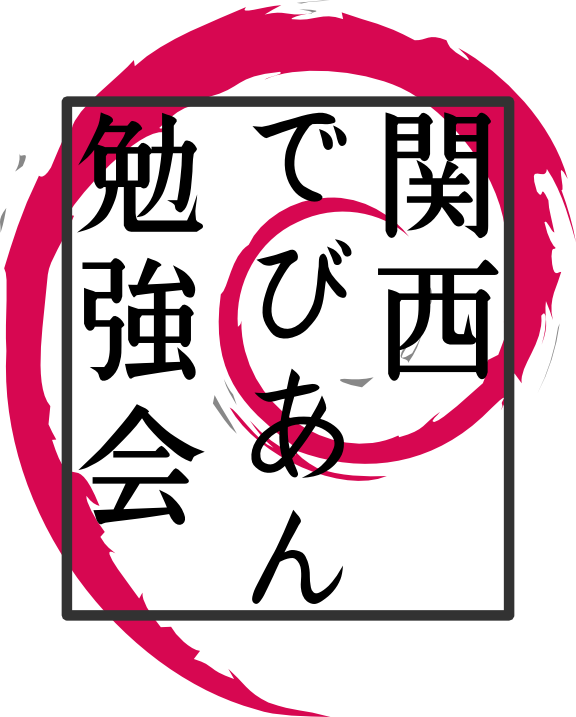
\includegraphics{image200802/kansaidebianlogo.png}
\end{center}

\begin{flushright}
\hfill{}関西 Debian 勉強会担当者 佐々木・倉敷・のがた・かわだ・八津尾 \\
\hfill{}\debmtgyear{}年\debmtgmonth{}月\debmtgdate{}日
\end{flushright}

\thispagestyle{empty}
\end{titlepage}

\dancersection{Introduction}{Debian JP}

\vspace{1em}

 関西Debian勉強会はDebian GNU/Linuxのさまざまなトピック
 (新しいパッケージ、Debian特有の機能の仕組、Debian界隈で起こった出来事、
 などなど)について話し合う会です。

 目的として次の三つを考えています。
 \begin{itemize}
  \item MLや掲示板ではなく、直接顔を合わせる事での情報交換の促進
  \item 定期的に集まれる場所
  \item 資料の作成
 \end{itemize}

 それでは、楽しい一時をお過ごしください。

\newpage

\begin{minipage}[b]{0.2\hsize}
 {\rotatebox{90}{\fontsize{80}{80}
{\gt 関西 Debian 勉強会}}}
\end{minipage}
\begin{minipage}[b]{0.8\hsize}
\hrule
\vspace{2mm}
\hrule
\setcounter{tocdepth}{1}
\tableofcontents
\vspace{2mm}
\hrule
\end{minipage}

\dancersection{最近のDebian関係のイベント報告}{Debian JP}

\subsection{第88回関西Debian勉強会}

88回目の関西Debian勉強会は9月28日(日)に、福島区民センターで行なわれました。

もくもくの会を中心とした内容での開催でした。

\subsection{第118回東京エリアDebian勉強会/オープンソースカンファレンス2014 Tokyo/Fall}

118回目の東京エリアDebian勉強会は10月18日(土)のOSC 2014 Tokyo/Fallで出
張開催されました。

岩松さんによる「Debian update」のセッションとブースの出展が行なわれまし
た。

\subsection{第119回東京エリアDebian勉強会x関東 LibreOffice オフxJessieインストーラテスト会、2014年10月 2nd勉強会}

119回目の東京エリアDebian勉強会は10月25日(土)に株式会社スクウェア・エニッ
クス セミナールームで開催されました。

10月2回目となる開催内容は、LibreOfficeとの合同開催でした。

\subsection{Debian Project}

\begin{itemize}
\item Re-Proposal - preserve freedom of choice of init systems \footnote{\url{https://lists.debian.org/debian-vote/2014/10/msg00001.html}}
\item \debianbug{66801} debootstrap: cant install systemd instead of sysvinit
\item apt-cudf \footnote{\url{https://lists.debian.org/debian-devel/2014/10/msg00480.html}}
\item apt-get purge chromium \footnote{\url{http://www.iuculano.it/linux/apt-get-purge-chromium/}}
\end{itemize}

\dancersection{事前課題}{Debian JP}

今回の課題は以下の通りです。
\begin{screen}
  \begin{enumerate}

  \item %
    もくもくの会で行なう作業、質問などの課題を用意して教えてください。
    (電源とネットワーク(WiMAXなど)はありますが、それ以外の作業に必要な
    環境はご用意ください。)

  \item %
    前回(第88回)の勉強会に参加された方は、前回の作業や課題がその後どう
    なったか結果を教えてください。

  \item %
    LT(ライトニングトーク) 歓迎です。何かお話したい方はタイトルを下さい。

  \end{enumerate}
\end{screen}

参加者の皆さんの解答は以下の通りです:

\begin{prework}{ kozo2 }
\end{prework}

\begin{prework}{ yyatsuo }
\end{prework}

\begin{prework}{ かわだてつたろう }
  \begin{enumerate}
  \item オレオレバックポートパッケージを作る。
  \end{enumerate}
\end{prework}

\begin{prework}{ 山城の国の住人 久保博 }

  \begin{enumerate}
  \item 前回宿題の続き。

    バッケージ引き取りの相談

    パッケージ作成方法のおさらい

  \item 前回宿題はまったく進捗なしです

  \end{enumerate}
\end{prework}

\begin{prework}{ 佐々木洋平 }
  \begin{enumerate}
  \item pkg-ruby-extras 関連の更新。...とtDiary。あと ibus-skk のデバッグ?
  \item 同上。
  \item systemd 無しで jessie を使うには、みたいなネタをできたら良いな、と思います。
  \end{enumerate}
\end{prework}

\begin{prework}{ lurdan }
  ちょっと顔を出すだけに、なる、かも
\end{prework}

\begin{prework}{ 川江 }
  \begin{enumerate}
  \item JavaScriptによるサイトのビルド。systemdとsysvinitの関係について
  \item 進捗は悪いです。
  \end{enumerate}
\end{prework}

\dancersection{もくもくの会}{}

\dancersection{今後の予定}{Debian JP}

\subsection{関西Debian勉強会}

次回、第90回関西Debian勉強会は11月8日(土)の関西オープンソース2014に出張
開催します。佐々木さんによる「Debian 8 "jessie" frozen」と題したセッショ
ンとブース出展の予定です。


\subsection{東京エリアDebian勉強会}

第120回東京エリアDebian勉強会は11月15日(土)に開催予定です。
場所、内容については東京エリアDebian勉強会のウェブサイトを確認してくだ
さい。

%
% 冊子にするために、4の倍数にする必要がある。
% そのための調整
%% \dancersection{メモ}{}
%% \mbox{}\newpage
%% \mbox{}\newpage
%% \mbox{}\newpage

\printindex
%\cleartooddpage

 \begin{minipage}[b]{0.2\hsize}
  \rotatebox{90}{\fontsize{80}{80} {\gt 関西 Debian 勉強会} }
 \end{minipage}
 \begin{minipage}[b]{0.8\hsize}

 \vspace*{15cm}
 \rule{\hsize}{1mm}
 \vspace{2mm}
 
\includegraphics[width=2cm]{image200502/openlogo-nd.eps}
 \noindent \Large \bfseries{Debian 勉強会資料}\\ \\
 \noindent \normalfont \debmtgyear{}年\debmtgmonth{}月\debmtgdate{}日 \hspace{5mm}  初版第1刷発行\\
 \noindent \normalfont 関西 Debian 勉強会 (編集・印刷・発行)\\
 \rule{\hsize}{1mm}
 \end{minipage}

\end{document}
